% Header: Here are all packages used and some additional definitions
%%%%%%%%%%%%%%%%%%%%%%%%%%%%%%%%%%%%%%%%%%%%%%%%%%%%%%%%%%%%%%%%%%%
\documentclass[11pt,a4paper]{scrartcl}
\usepackage[margin=2.5cm]{geometry}
\usepackage[onehalfspacing]{setspace}
\usepackage{graphicx} % zum Einbinden von Graphiken
\usepackage{float}
\usepackage[ngerman]{babel}
\usepackage[font=footnotesize, bf, format=plain, font=normalsize]{caption}
\usepackage{graphicx}
\usepackage{wrapfig}
\usepackage[hidelinks]{hyperref} % f. Referenzen
\usepackage{amsmath,amsthm,amssymb} % Mathematik Umgebung 
\usepackage{icomma} % Intelligentes Komma, das den richtigen Abstand zwischen Dezimalzahlen als auch in Formeln wählt.
\usepackage[ngerman]{babel} % Deutsche Bezeichnungen bei Inhaltsangabe etc
%\usepackage[T1]{fontenc}    % andere Schriftsatzkodierung für richtige Silbentrennung bei Umlauten
\usepackage[locale = DE,space-before-unit=true,per-mode = fraction]{siunitx} % Bessere Einheiten
\usepackage{booktabs,multirow} % Pakete zur Erstellung von Tabellen
\usepackage{placeins} % Definiert den Befehl “\FloatBarrier”, der die Ausgabe der davor eingebundenen Bilder erzwingt, befor der Text weiter geht. (Mit vorsicht zu verwenden)
\usepackage[backend=biber,abbreviate=true,doi=false,style=numeric-comp,giveninits=true,sorting=none]{biblatex} % Modernes Paket zur Erzeugung von Bibliografien (benötigt biber!)
\usepackage{csquotes} % Fortgeschrittene Funktionen für Zitate, für die deutsche Form der Anführungszeichen bei Referenzen
\usepackage[dvipsnames]{xcolor}
\addbibresource{MyBibliography.bib} % Ort der .bib Datei, die die Datenbank für Literatur/Referenzen enthält.

\graphicspath{{bilder/}}

% place eqn number in brackets for autoref
\makeatletter
\def\tagform@#1{\maketag@@@{\ignorespaces#1\unskip\@@italiccorr}}
\let\orgtheequation\theequation
\def\theequation{(\orgtheequation)}
\makeatother

\definecolor{MyBlue}{HTML}{0072B2}
\definecolor{MyOrange}{HTML}{D55E00}
\definecolor{MyRed}{HTML}{F00F0F}

\hypersetup{%
%	colorlinks=true,
	breaklinks=true,
	linkcolor=blue,
	urlcolor=blue,
	citecolor=blue,
	linkbordercolor={0 0 1}
}

\let\oldunit\unit
\renewcommand{\unit}[1]{\hspace{4pt}\oldunit{#1}}

\DeclareSIUnit{\dBm}{dBm}
\DeclareSIUnit[per-mode=reciprocal]\WN{\per\centi\meter}

%%%%%%%%%%%%%%%%%%%%%%%%%%%%%%%%%%%%%%%%%%%%%%%%%%%%%%%%%%%%%%%%%%%
\begin{document}
%
\def\settitle{}
\thispagestyle{empty}
\titlehead{
\includegraphics[width=5cm]{logo.jpg}}
\title{\settitle}
\author{Alexander Helbok\thanks{\href{mailto:alexander.helbok@student.uibk.ac.at}{alexander.helbok@student.uibk.ac.at}},
		Jakob Höck \thanks{\href{mailto:jakob.hoeck@student.uibk.ac.at}{jakob.hoeck@student.uibk.ac.at}},
		Max Koppelstätter\thanks{\href{mailto:max.koppelstaetter@student.uibk.ac.at}{max.koppelstaetter@student.uibk.ac.at}}}
\date{\today}
\maketitle
\vfill



\section*{Abstract}
Dieser Versuch beschäftigt sich mit der Funktionsweise eines Halbleiters sowie dem Hall-Effekt. Dabei wird die van-der-Pauw-Methode angewandt, um den spezifischen Widerstand sowie den Hall-Koeffizienten eines Halbleiters zu bestimmen. Eine Halbleiter-Probe wird in einem Kryostaten von Raumtemperatur ausgehend bis etwa 20 K abgekühlt. Während des Abkühlvorgangs werden die genannten Eigenschaften in kleinen Temperaturschritten aufgezeichnet, wodurch wir feststellen können, ob der Halbleiter n- oder p-dotiert ist. Aus diesen Daten lässt sich auch die Beweglichkeit der Ladungsträger, die Ionisierungsenergie der Donatoren bzw. Akzeptoren, sowie die Streumechanismen im Halbleiter bestimmen. Es wird eine direkte Beobachtung der Matthiessenschen Regel diskutiert, sowie festgestellt, dass es sich bei dem zu untersuchenden Material um n-dotiertes Galliumarsenid handelt.
\vspace{1cm}
\newpage
%
%
\tableofcontents
\cleardoublepage
\pagenumbering{arabic} 
%
%
\setcounter{section}{-1}
\section{Einleitung}


\section{Theorie}
\label{sec:theorie}

%\begin{figure}[H]
%    \centering
%    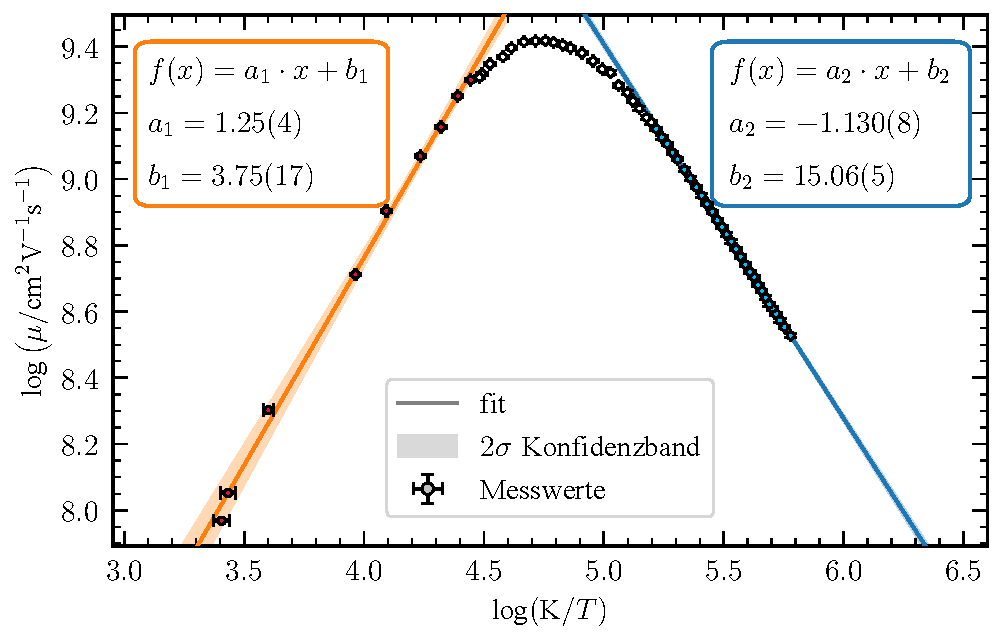
\includegraphics[width=\textwidth]{plot3.pdf}
%    \caption{}
%    \label{fig:plot3}
%\end{figure}


\input{03_Durchführung}

\section{Ergebnisse}

%\begin{figure}[H]
%    \centering
%    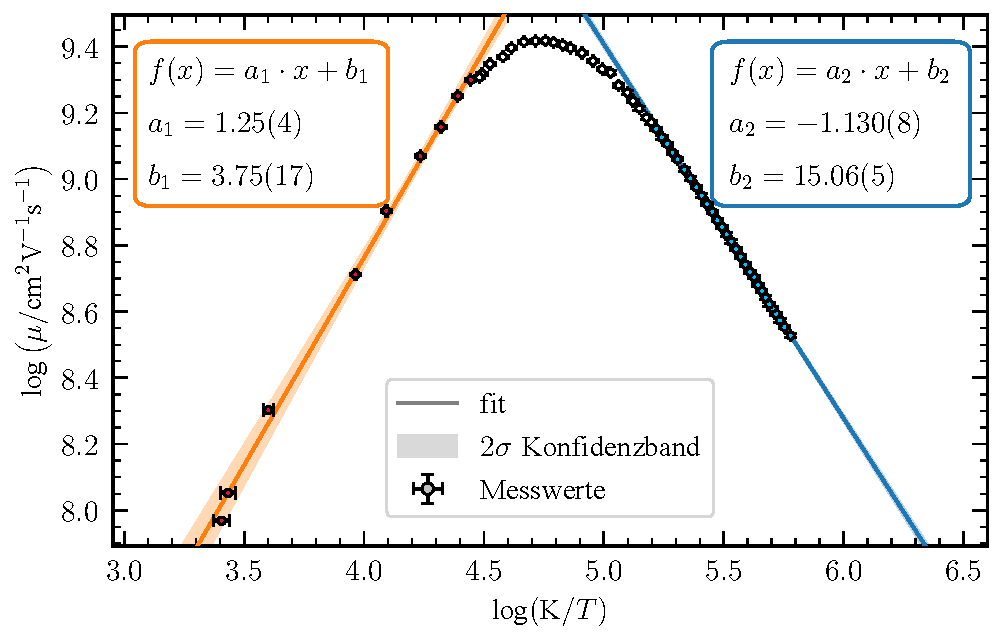
\includegraphics[width=\textwidth]{plot3.pdf}
%    \caption{}
%    \label{fig:plot3}
%\end{figure}


\section{Schlussfolgerung}
 

%\input{Anhang} % Der Anhang ist in einer externen Datei "Anhang.tex" und wird hier in das Dokument eingefügt.

\newpage

\printbibliography
%\vfill
\clearpage

\section*{Erklärung}

Hiermit versichern wir, dass der vorliegende Bericht selbständig verfasst wurde und alle notwendigen Quellen und Referenzen angegeben sind.

\begin{tabular}{@{}p{2.5in}p{2.5in}@{}}
    \\[5\bigskipamount]
    & \hspace{2mm}\today \\[-12pt]
    \dotfill & \dotfill \\
    Alexander Helbok & Date \\[5\bigskipamount]
    & \hspace{2mm}\today \\[-12pt]
    \dotfill & \dotfill \\
    Jakob Hugo Höck & Date \\
    [5\bigskipamount]
    & \hspace{2mm}\today \\[-12pt]
    \dotfill & \dotfill \\
    Max Koppelstätter & Date \\
    \centering
\end{tabular}

\begin{minipage}{0.3\textwidth}
	\vspace{-18.5cm}
	
\includegraphics[scale=0.3]{alex_sign}
\end{minipage}

\begin{minipage}{0.3\textwidth}
	\vspace{-12cm}
	
\includegraphics[scale=1]{UnterschriftHugo}
\end{minipage}

\begin{minipage}{0.3\textwidth}
	\vspace{-6.7cm}
	
\includegraphics[scale=0.2]{max_sign}
\end{minipage}

\end{document}
